\section{Analysis}

As said in Section 3, we will follow the Performance Optimization and Productivity. The POP Efficiency metrics are the base of the methodology. First, we usually run the application many times in a \textit{strong scaling} manner. Strong scaling means leaving the problem's size constant and increasing the resources, for example, running the same Alya input set with 1, 2, 4 and Nodes. Then we gather necessary data for computing the efficiency metrics from the previous runs. Once we have the metrics, we possess insight into the factors limiting the code's performance when scaling in the number of resources. From this insight, we can locate the zones in the code responsible for it and try to propose a better implementation.

\subsection{Efficiency metrics}

\begin{figure}[htbp]
\centering
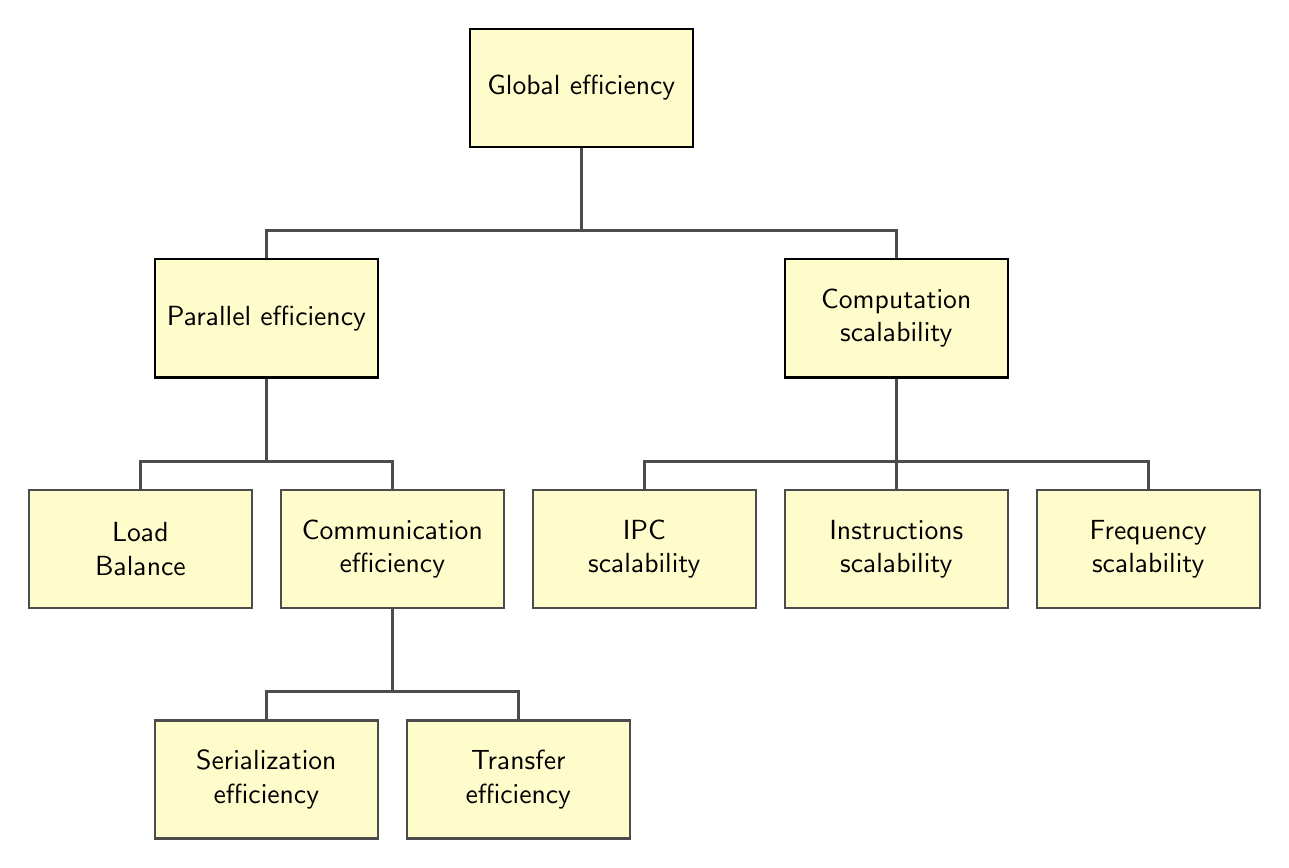
\begin{tikzpicture}[
% Label style
    label distance=3mm,
    every label/.style={blue},
% Event style
    event/.style={rectangle,thick,draw,fill=yellow!20,text width=2.6cm, minimum height=1.5cm,
		text centered,font=\sffamily,anchor=north},
% Children and edges style
    edge from parent/.style={very thick,draw=black!70},
    edge from parent path={(\tikzparentnode.south) -- ++(0,-1.05cm)
			-| (\tikzchildnode.north)},
    level 1/.style={sibling distance=8cm,level distance=1.4cm,
			growth parent anchor=south,nodes=event},
    level 2/.style={sibling distance=3.2cm},
    level 3/.style={sibling distance=3.2cm},
    level 4/.style={sibling distance=1cm}
%%  For compatability with PGF CVS add the absolute option:
%   absolute
    ]

  \node (glob) [event] {Global efficiency}
    child{node (par) {Parallel efficiency}
      child {node (lb) {Load  \\ Balance}}
      child {node (comm) {Communication efficiency}
        child {node (ser) {Serialization efficiency}}
        child {node (trans) {Transfer efficiency}}
      }
    }
    child{node (comp) {Computation scalability}
      child{node (ipc) {IPC \\ scalability}}
      child{node (ins) {Instructions scalability}}
      child{node (fre) {Frequency scalability}}
    };
\end{tikzpicture}
\caption{POP Efficiency metrics}
\label{popmet}
\end{figure}
